\chapter[Définition du sujet]{Définition du sujet}

\textit{Le présent chapitre a pour objectif de définir le sujet : cela permettra de préciser le contexte de l'étude et de redéfinir la problématique, avant d'analyser les enjeux du projet. }

\section{Contexte du sujet}

Grâce au développement des techniques LiDAR et aux prises de vues aériennes et satellites, il est possible de représenter le terrain (création de Modèles Numériques de Terrain). Afin d'avoir une bonne maitrise du milieu urbain, le processus de reconstruction 3D permet d'avoir une modélisation plus avancée. Pour construire ces maquettes 3D urbaines, on utilise un nuage de points, créé à partir de données LiDAR ou par reconstruction photogrammétrique. \newline

\begin{figure}[H]
	\begin{center}
		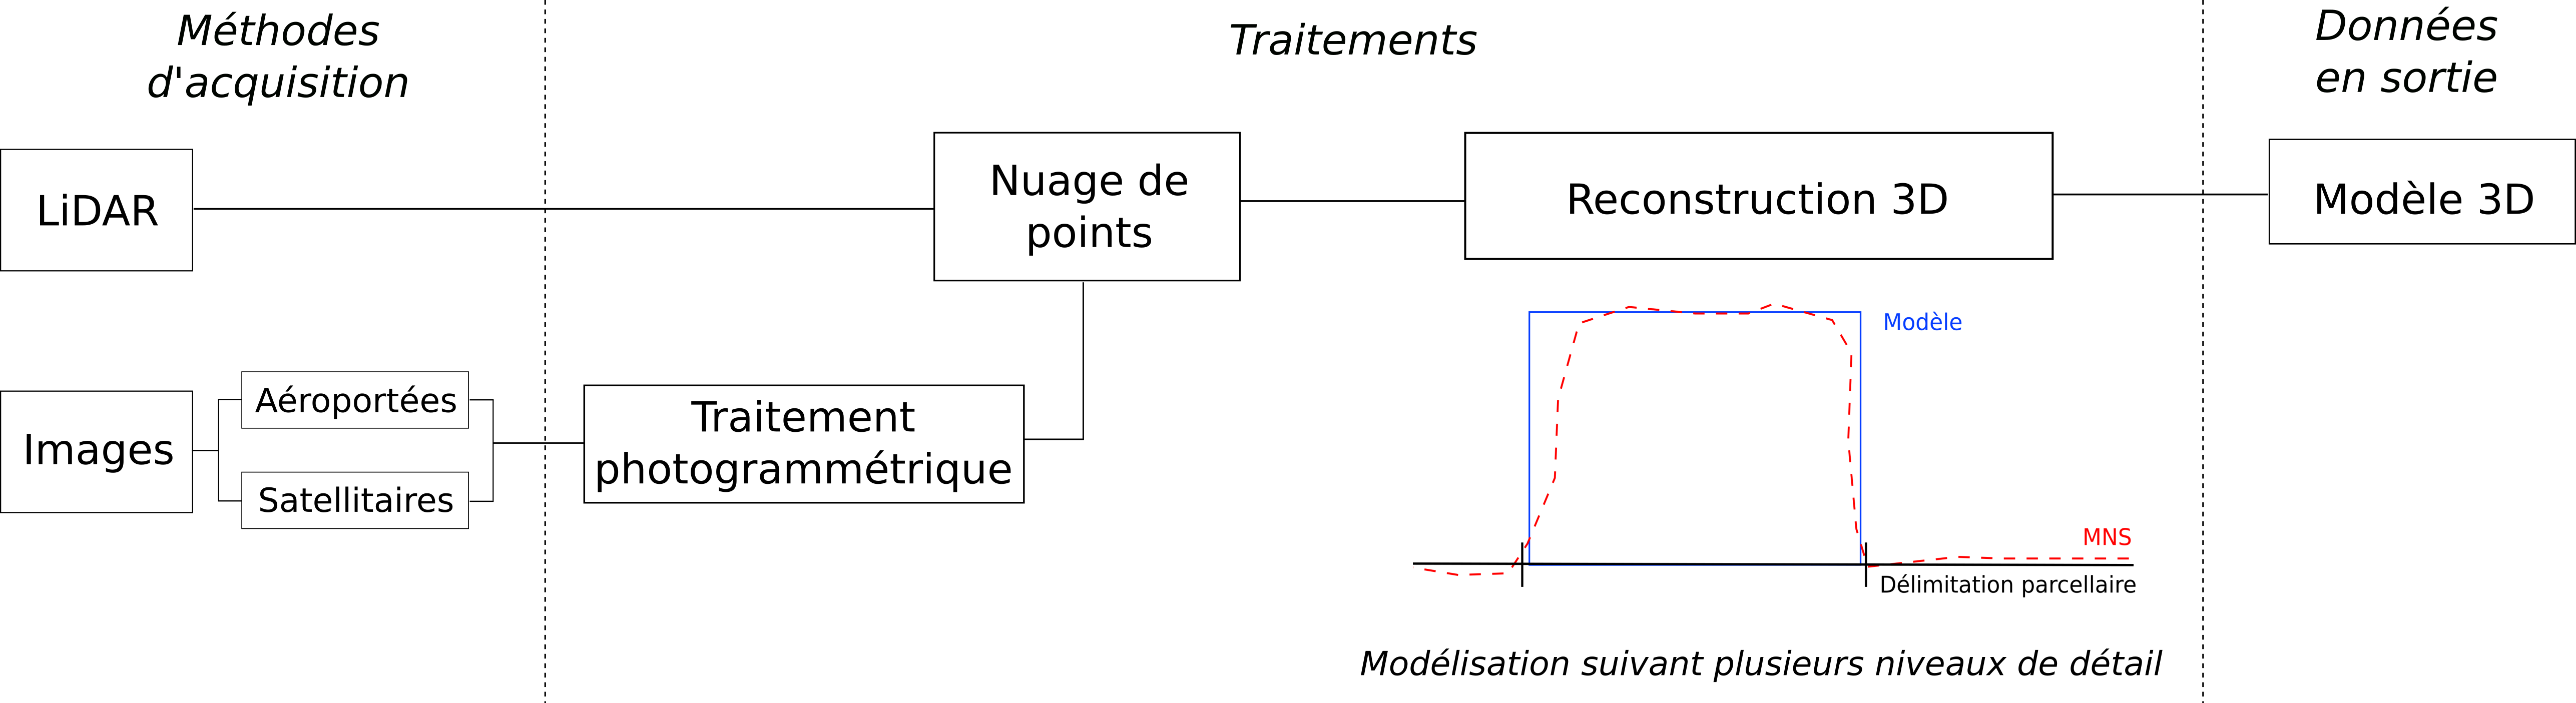
\includegraphics[scale=0.38]{Process_ini.png}  \\
		\caption[Chaîne simplifiée de reconstruction 3D urbaine]{Chaîne simplifiée de reconstruction 3D urbaine}
		\label{fig:recons3D}
	\end{center}
\end{figure}

\begin{figure}[H]
	\begin{center}
		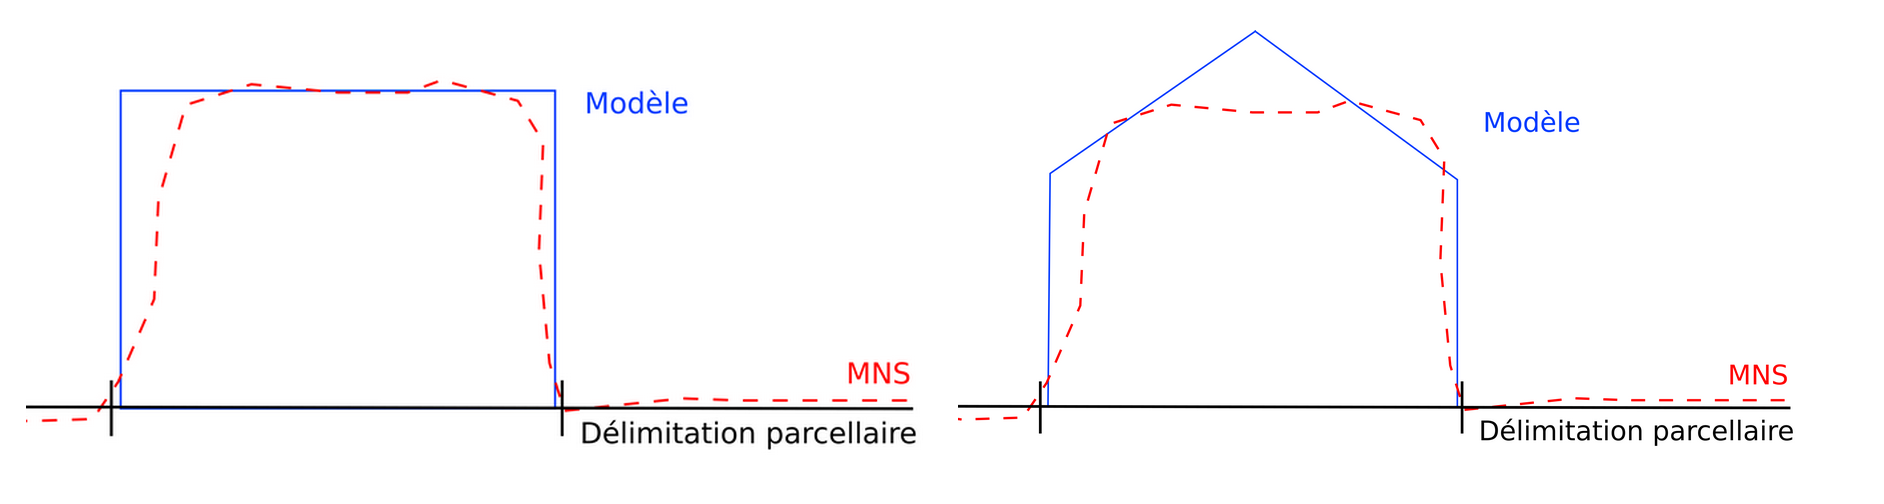
\includegraphics[scale=0.32]{Correlation.png}  \\
		\caption[Principe de la reconstruction urbaine]{Principe de la reconstruction urbaine}
		\label{fig:correlobj}
	\end{center}
\end{figure}

\newpage
Le niveau de détail de la maquette (LoD) peut varier selon les objectifs de l'utilisateur. Différentes modélisations sont possibles : 
\begin{itemize}[label=$\rightarrow$]
	\item Manhattan (LoD1 = toits plats)
	\item Biplan (LoD2 = toits pentus)
	\item Modélisation précise (LoD3 = représentation des microstructures - cheminées, gouttières, ...) 
\end{itemize}
Plus le modèle est évolué, plus le niveau de détail est important mais plus la généralisation est compliquée.\newline


\begin{figure}[!h]
	\begin{center}
		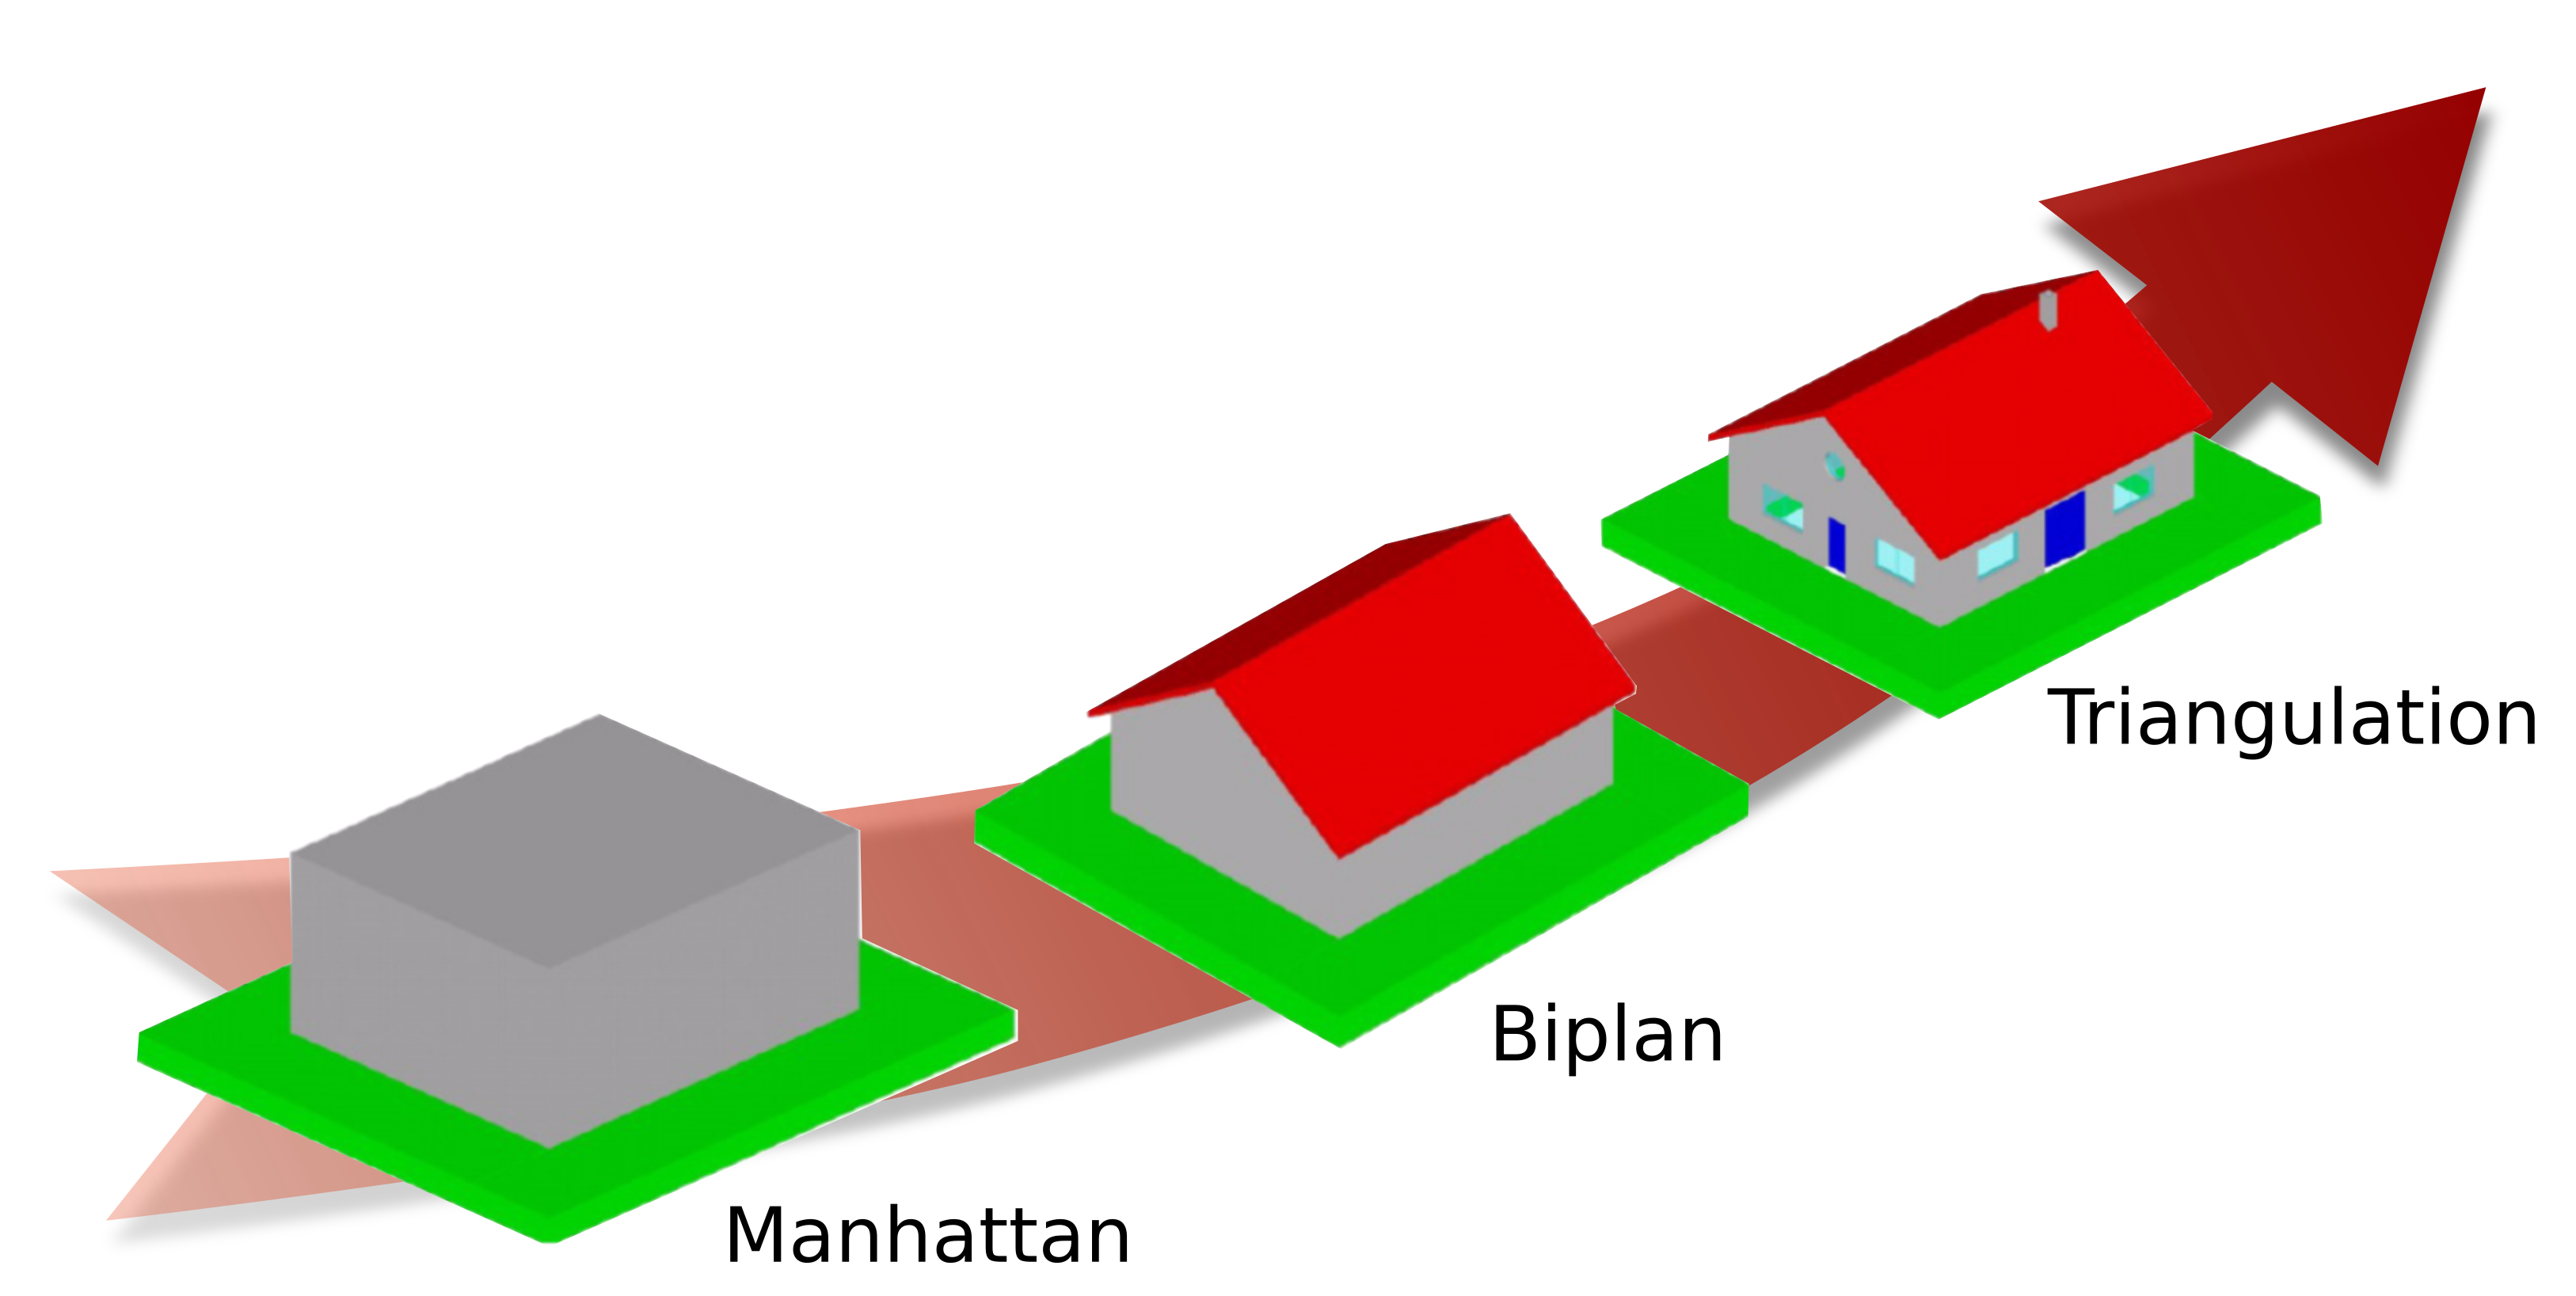
\includegraphics[scale=0.15]{Niveau_detail.png}  \\
		\caption[Impact du niveau de détail sur la modélisation]{Impact du niveau de détail sur la modélisation\footnotemark{}}
		\label{fig:LOD}
	\end{center}
\end{figure}
\footnotetext{Sources : OGC CityGML Implementation Specification 1 (Research Center Karlsruhe)}

Aujourd'hui, les techniques de reconstruction automatiques ne sont pas opérationnelles. L’utilisateur doit intervenir pour corriger manuellement les erreurs. Le passage à l'échelle de la chaîne de production devient donc problématique. Afin d'alléger la phase de correction, on cherche à automatiser la qualification de ces modèles. Pour cela, deux méthodes sont envisageables : la qualification avec des données de référence (nécessite un modèle de référence), et l’auto-qualification. \newline

En matière de reconstruction 3D, le laboratoire MATIS de l'IGN a mis au point la méthode de reconstruction automatique BATI-3D. Le projet présenté ici s’inscrit dans le cadre des recherches du laboratoire pour la reconstruction 3D des bâtiments à partir de Modèles Numériques de Surface (MNS). L'objectif est d'automatiser la correction des maquettes 3D urbaines. Cela implique d'automatiser en premier la phase d'auto-qualification des erreurs.

\section{Problématique}

Pour détecter et caractériser les erreurs de reconstruction, l’équipe de recherche a mis en place une méthode d'auto-qualification. Ce processus passe par la réalisation d'une classification supervisée des entités reconstruites, afin de leur associer une classe d'erreur. \newline

Les différents types d'erreur sont ordonnés hiérarchiquement selon des classes, choisies en fonction du niveau de détail de la reconstruction. Ainsi, on peut définir une typologie des erreurs rencontrées (cf. annexe \ref{annexeerreurs}).\newline

L'objectif du projet est d'évoluer vers une classification active. En effet, l'intervention d'un utilisateur permettrait de valider (ou non) les résultats de la classification, afin d'affiner le modèle de prédiction entrainé.\newline
 
Le projet de développement présenté dans ce rapport propose donc de mettre en place un outil graphique d'aide à la classification active. L'objectif est de réaliser une interface permettant à un utilisateur de valider un résultat de classification, ou dans le cas contraire de renseigner la bonne erreur. Pour cela, les objets d'intérêt (orthophoto et bâtiments orthoprojetés) doivent pouvoir être visualisés selon une hiérarchie à définir.\newline

\begin{figure}[!h]
	\begin{center}
		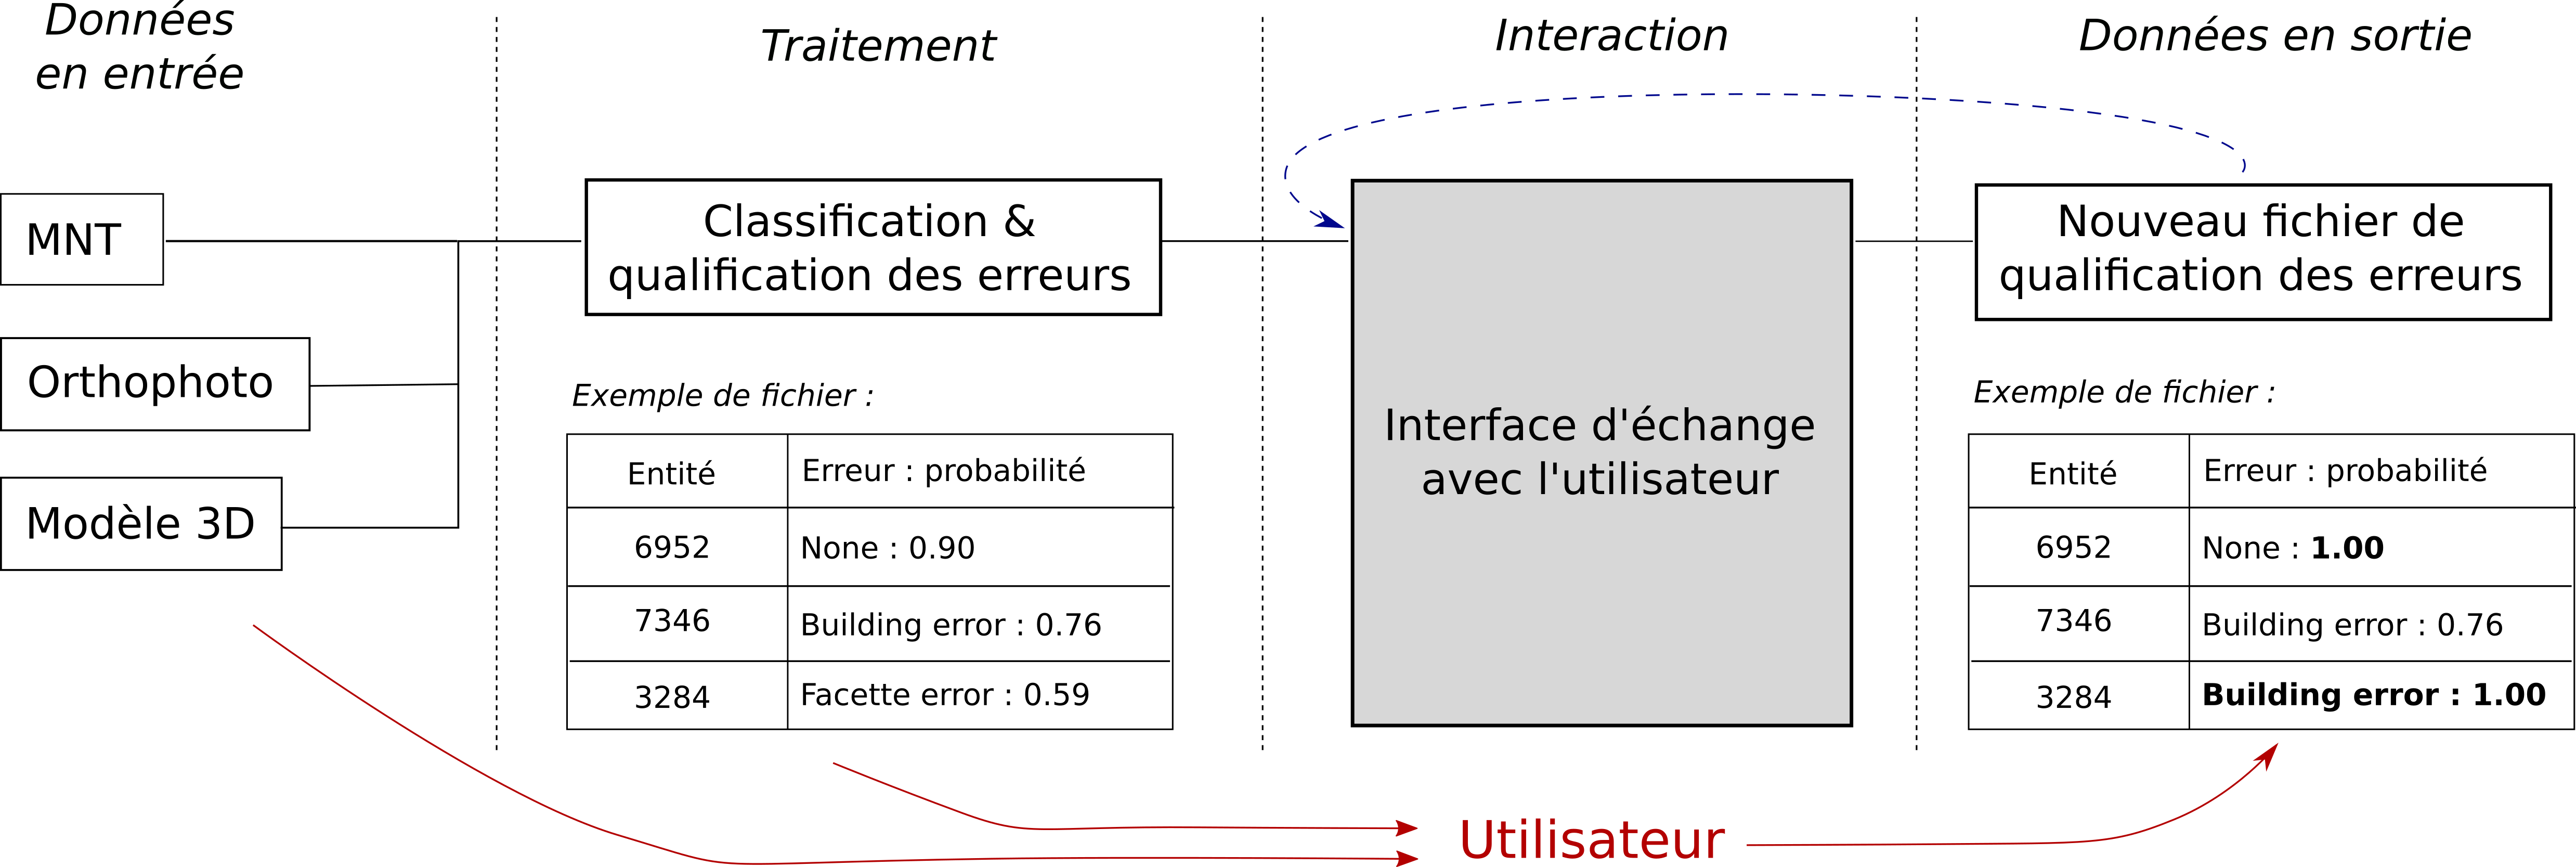
\includegraphics[scale=0.38]{Process_projet.png}  \\
		\caption[Chaîne de traitement simplifiée du projet]{Chaîne de traitement simplifiée du projet}
		\label{fig:processprojet}
	\end{center}
\end{figure}

\section{Analyse des besoins}

Après avoir défini précisément le contexte du projet et sa problématique, il est possible d'analyser ses principaux objectifs. Ainsi, les enjeux du projet sont liés à l'affichage et à la validation des résultats de la classification.

\begin{figure}[!h]
	\begin{center}
		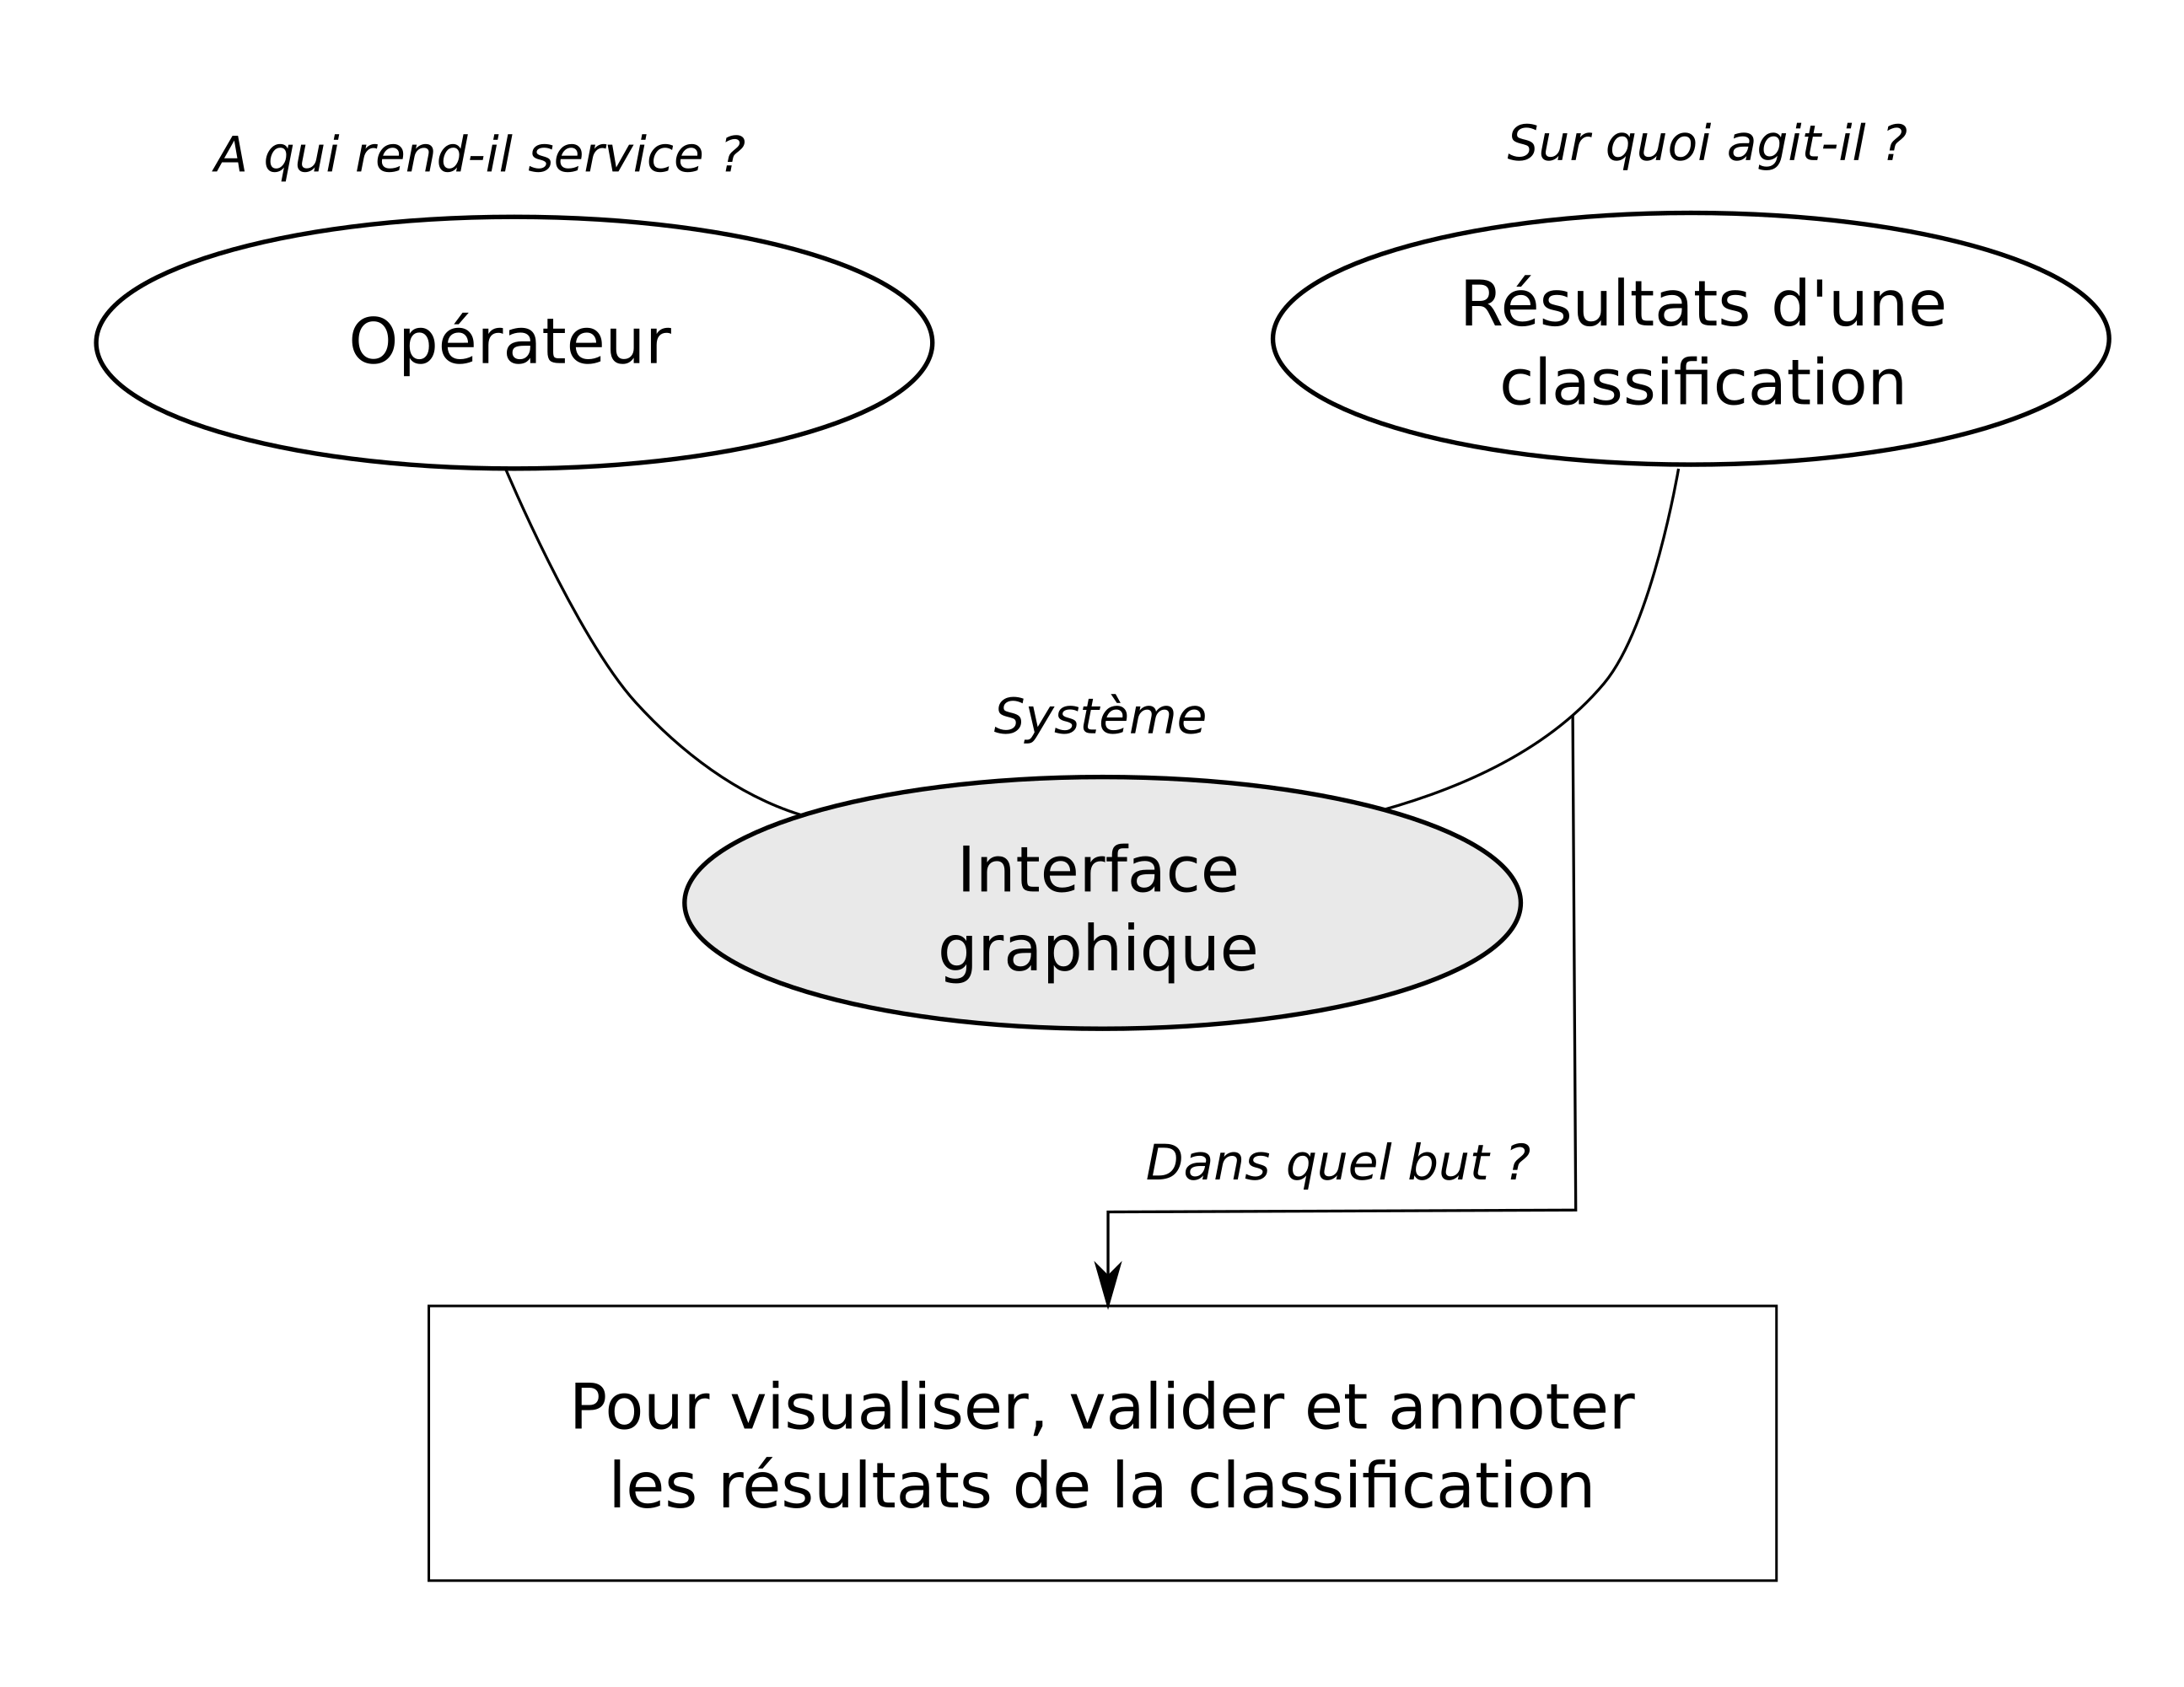
\includegraphics[scale=0.45]{Bete_corne.png}  \\
		\caption[Objectifs généraux du projet]{Objectifs généraux du projet}
		\label{fig:betecorne}
	\end{center}
\end{figure}

Dans un premier temps,ce projet s'adresse aux utilisateurs du processus de qualification des données de reconstruction 3D urbaine. Cependant, l'interface réalisée peut être amenée à évoluer et à servir pour visualiser d'autres cas de classification. 
